\documentclass[1p]{elsarticle_modified}
%\bibliographystyle{elsarticle-num}

%\usepackage[colorlinks]{hyperref}
%\usepackage{abbrmath_seonhwa} %\Abb, \Ascr, \Acal ,\Abf, \Afrak
\usepackage{amsfonts}
\usepackage{amssymb}
\usepackage{amsmath}
\usepackage{amsthm}
\usepackage{scalefnt}
\usepackage{amsbsy}
\usepackage{kotex}
\usepackage{caption}
\usepackage{subfig}
\usepackage{color}
\usepackage{graphicx}
\usepackage{xcolor} %% white, black, red, green, blue, cyan, magenta, yellow
\usepackage{float}
\usepackage{setspace}
\usepackage{hyperref}

\usepackage{tikz}
\usetikzlibrary{arrows}

\usepackage{multirow}
\usepackage{array} % fixed length table
\usepackage{hhline}

%%%%%%%%%%%%%%%%%%%%%
\makeatletter
\renewcommand*\env@matrix[1][\arraystretch]{%
	\edef\arraystretch{#1}%
	\hskip -\arraycolsep
	\let\@ifnextchar\new@ifnextchar
	\array{*\c@MaxMatrixCols c}}
\makeatother %https://tex.stackexchange.com/questions/14071/how-can-i-increase-the-line-spacing-in-a-matrix
%%%%%%%%%%%%%%%

\usepackage[normalem]{ulem}

\newcommand{\msout}[1]{\ifmmode\text{\sout{\ensuremath{#1}}}\else\sout{#1}\fi}
%SOURCE: \msout is \stkout macro in https://tex.stackexchange.com/questions/20609/strikeout-in-math-mode

\newcommand{\cancel}[1]{
	\ifmmode
	{\color{red}\msout{#1}}
	\else
	{\color{red}\sout{#1}}
	\fi
}

\newcommand{\add}[1]{
	{\color{blue}\uwave{#1}}
}

\newcommand{\replace}[2]{
	\ifmmode
	{\color{red}\msout{#1}}{\color{blue}\uwave{#2}}
	\else
	{\color{red}\sout{#1}}{\color{blue}\uwave{#2}}
	\fi
}

\newcommand{\Sol}{\mathcal{S}} %segment
\newcommand{\D}{D} %diagram
\newcommand{\A}{\mathcal{A}} %arc


%%%%%%%%%%%%%%%%%%%%%%%%%%%%%5 test

\def\sl{\operatorname{\textup{SL}}(2,\Cbb)}
\def\psl{\operatorname{\textup{PSL}}(2,\Cbb)}
\def\quan{\mkern 1mu \triangleright \mkern 1mu}

\theoremstyle{definition}
\newtheorem{thm}{Theorem}[section]
\newtheorem{prop}[thm]{Proposition}
\newtheorem{lem}[thm]{Lemma}
\newtheorem{ques}[thm]{Question}
\newtheorem{cor}[thm]{Corollary}
\newtheorem{defn}[thm]{Definition}
\newtheorem{exam}[thm]{Example}
\newtheorem{rmk}[thm]{Remark}
\newtheorem{alg}[thm]{Algorithm}

\newcommand{\I}{\sqrt{-1}}
\begin{document}

%\begin{frontmatter}
%
%\title{Boundary parabolic representations of knots up to 8 crossings}
%
%%% Group authors per affiliation:
%\author{Yunhi Cho} 
%\address{Department of Mathematics, University of Seoul, Seoul, Korea}
%\ead{yhcho@uos.ac.kr}
%
%
%\author{Seonhwa Kim} %\fnref{s_kim}}
%\address{Center for Geometry and Physics, Institute for Basic Science, Pohang, 37673, Korea}
%\ead{ryeona17@ibs.re.kr}
%
%\author{Hyuk Kim}
%\address{Department of Mathematical Sciences, Seoul National University, Seoul 08826, Korea}
%\ead{hyukkim@snu.ac.kr}
%
%\author{Seokbeom Yoon}
%\address{Department of Mathematical Sciences, Seoul National University, Seoul, 08826,  Korea}
%\ead{sbyoon15@snu.ac.kr}
%
%\begin{abstract}
%We find all boundary parabolic representation of knots up to 8 crossings.
%
%\end{abstract}
%\begin{keyword}
%    \MSC[2010] 57M25 
%\end{keyword}
%
%\end{frontmatter}

%\linenumbers
%\tableofcontents
%
\newcommand\colored[1]{\textcolor{white}{\rule[-0.35ex]{0.8em}{1.4ex}}\kern-0.8em\color{red} #1}%
%\newcommand\colored[1]{\textcolor{white}{ #1}\kern-2.17ex	\textcolor{white}{ #1}\kern-1.81ex	\textcolor{white}{ #1}\kern-2.15ex\color{red}#1	}

{\Large $\underline{12a_{0544}~(K12a_{0544})}$}

\setlength{\tabcolsep}{10pt}
\renewcommand{\arraystretch}{1.6}
\vspace{1cm}\begin{tabular}{m{100pt}>{\centering\arraybackslash}m{274pt}}
\multirow{5}{120pt}{
	\centering
	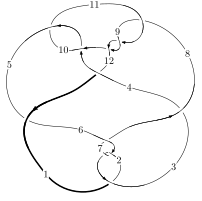
\includegraphics[width=112pt]{../../../GIT/diagram.site/Diagrams/png/1345_12a_0544.png}\\
\ \ \ A knot diagram\footnotemark}&
\allowdisplaybreaks
\textbf{Linearized knot diagam} \\
\cline{2-2}
 &
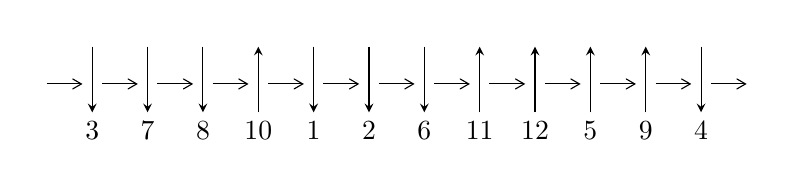
\begin{tikzpicture}[x=20pt, y=17pt]
	% nodes
	\node (C0) at (0, 0) {};
	\node (C1) at (1, 0) {};
	\node (C1U) at (1, +1) {};
	\node (C1D) at (1, -1) {3};

	\node (C2) at (2, 0) {};
	\node (C2U) at (2, +1) {};
	\node (C2D) at (2, -1) {7};

	\node (C3) at (3, 0) {};
	\node (C3U) at (3, +1) {};
	\node (C3D) at (3, -1) {8};

	\node (C4) at (4, 0) {};
	\node (C4U) at (4, +1) {};
	\node (C4D) at (4, -1) {10};

	\node (C5) at (5, 0) {};
	\node (C5U) at (5, +1) {};
	\node (C5D) at (5, -1) {1};

	\node (C6) at (6, 0) {};
	\node (C6U) at (6, +1) {};
	\node (C6D) at (6, -1) {2};

	\node (C7) at (7, 0) {};
	\node (C7U) at (7, +1) {};
	\node (C7D) at (7, -1) {6};

	\node (C8) at (8, 0) {};
	\node (C8U) at (8, +1) {};
	\node (C8D) at (8, -1) {11};

	\node (C9) at (9, 0) {};
	\node (C9U) at (9, +1) {};
	\node (C9D) at (9, -1) {12};

	\node (C10) at (10, 0) {};
	\node (C10U) at (10, +1) {};
	\node (C10D) at (10, -1) {5};

	\node (C11) at (11, 0) {};
	\node (C11U) at (11, +1) {};
	\node (C11D) at (11, -1) {9};

	\node (C12) at (12, 0) {};
	\node (C12U) at (12, +1) {};
	\node (C12D) at (12, -1) {4};
	\node (C13) at (13, 0) {};

	% arrows
	\draw[->,>={angle 60}]
	(C0) edge (C1) (C1) edge (C2) (C2) edge (C3) (C3) edge (C4) (C4) edge (C5) (C5) edge (C6) (C6) edge (C7) (C7) edge (C8) (C8) edge (C9) (C9) edge (C10) (C10) edge (C11) (C11) edge (C12) (C12) edge (C13) ;	\draw[->,>=stealth]
	(C1U) edge (C1D) (C2U) edge (C2D) (C3U) edge (C3D) (C4D) edge (C4U) (C5U) edge (C5D) (C6U) edge (C6D) (C7U) edge (C7D) (C8D) edge (C8U) (C9D) edge (C9U) (C10D) edge (C10U) (C11D) edge (C11U) (C12U) edge (C12D) ;
	\end{tikzpicture} \\
\hhline{~~} \\& 
\textbf{Solving Sequence} \\ \cline{2-2} 
 &
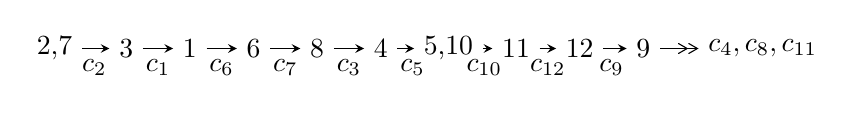
\begin{tikzpicture}[x=23pt, y=7pt]
	% node
	\node (A0) at (-1/8, 0) {2,7};
	\node (A1) at (1, 0) {3};
	\node (A2) at (2, 0) {1};
	\node (A3) at (3, 0) {6};
	\node (A4) at (4, 0) {8};
	\node (A5) at (5, 0) {4};
	\node (A6) at (97/16, 0) {5,10};
	\node (A7) at (57/8, 0) {11};
	\node (A8) at (65/8, 0) {12};
	\node (A9) at (73/8, 0) {9};
	\node (C1) at (1/2, -1) {$c_{2}$};
	\node (C2) at (3/2, -1) {$c_{1}$};
	\node (C3) at (5/2, -1) {$c_{6}$};
	\node (C4) at (7/2, -1) {$c_{7}$};
	\node (C5) at (9/2, -1) {$c_{3}$};
	\node (C6) at (11/2, -1) {$c_{5}$};
	\node (C7) at (53/8, -1) {$c_{10}$};
	\node (C8) at (61/8, -1) {$c_{12}$};
	\node (C9) at (69/8, -1) {$c_{9}$};
	\node (A10) at (11, 0) {$c_{4},c_{8},c_{11}$};

	% edge
	\draw[->,>=stealth]	
	(A0) edge (A1) (A1) edge (A2) (A2) edge (A3) (A3) edge (A4) (A4) edge (A5) (A5) edge (A6) (A6) edge (A7) (A7) edge (A8) (A8) edge (A9) ;
	\draw[->>,>={angle 60}]	
	(A9) edge (A10);
\end{tikzpicture} \\ 

\end{tabular} \\

\footnotetext{
The image of knot diagram is generated by the software ``\textbf{Draw programme}" developed by Andrew Bartholomew(\url{http://www.layer8.co.uk/maths/draw/index.htm\#Running-draw}), where we modified some parts for our purpose(\url{https://github.com/CATsTAILs/LinksPainter}).
}\phantom \\ \newline 
\centering \textbf{Ideals for irreducible components\footnotemark of $X_{\text{par}}$} 
 
\begin{align*}
I^u_{1}&=\langle 
u^{85}+u^{84}+\cdots+b+1,\;u^{85}+u^{84}+\cdots+a+3,\;u^{86}+2 u^{85}+\cdots+5 u+1\rangle \\
I^u_{2}&=\langle 
- u^7+u^5- u^3+b-1,\;- u^7+u^5- u^4- u^3+u^2+a-2,\;u^8- u^7- u^6+2 u^5+u^4-2 u^3+2 u-1\rangle \\
\\
\end{align*}
\raggedright * 2 irreducible components of $\dim_{\mathbb{C}}=0$, with total 94 representations.\\
\footnotetext{All coefficients of polynomials are rational numbers. But the coefficients are sometimes approximated in decimal forms when there is not enough margin.}
\newpage
\renewcommand{\arraystretch}{1}
\centering \section*{I. $I^u_{1}= \langle u^{85}+u^{84}+\cdots+b+1,\;u^{85}+u^{84}+\cdots+a+3,\;u^{86}+2 u^{85}+\cdots+5 u+1 \rangle$}
\flushleft \textbf{(i) Arc colorings}\\
\begin{tabular}{m{7pt} m{180pt} m{7pt} m{180pt} }
\flushright $a_{2}=$&$\begin{pmatrix}1\\0\end{pmatrix}$ \\
\flushright $a_{7}=$&$\begin{pmatrix}0\\u\end{pmatrix}$ \\
\flushright $a_{3}=$&$\begin{pmatrix}1\\u^2\end{pmatrix}$ \\
\flushright $a_{1}=$&$\begin{pmatrix}- u^2+1\\- u^4\end{pmatrix}$ \\
\flushright $a_{6}=$&$\begin{pmatrix}u\\u\end{pmatrix}$ \\
\flushright $a_{8}=$&$\begin{pmatrix}- u^3\\- u^3+u\end{pmatrix}$ \\
\flushright $a_{4}=$&$\begin{pmatrix}- u^8+u^6- u^4+1\\- u^8+2 u^6-2 u^4+2 u^2\end{pmatrix}$ \\
\flushright $a_{5}=$&$\begin{pmatrix}- u^7+2 u^5-2 u^3+2 u\\- u^9+u^7- u^5+u\end{pmatrix}$ \\
\flushright $a_{10}=$&$\begin{pmatrix}- u^{85}- u^{84}+\cdots+2 u^2-3\\- u^{85}- u^{84}+\cdots-2 u-1\end{pmatrix}$ \\
\flushright $a_{11}=$&$\begin{pmatrix}- u^{85}+u^{84}+\cdots+5 u-2\\-3 u^{85}- u^{84}+\cdots-3 u-1\end{pmatrix}$ \\
\flushright $a_{12}=$&$\begin{pmatrix}- u^{20}+3 u^{18}-7 u^{16}+10 u^{14}-10 u^{12}+7 u^{10}- u^8-2 u^6+3 u^4-3 u^2+1\\- u^{20}+4 u^{18}-10 u^{16}+18 u^{14}-23 u^{12}+24 u^{10}-18 u^8+10 u^6-5 u^4\end{pmatrix}$ \\
\flushright $a_{9}=$&$\begin{pmatrix}- u^{85}+14 u^{83}+\cdots+2 u-2\\-2 u^{85}- u^{84}+\cdots-2 u-1\end{pmatrix}$\\&\end{tabular}
\flushleft \textbf{(ii) Obstruction class $= -1$}\\~\\
\flushleft \textbf{(iii) Cusp Shapes $= - u^{85}+2 u^{84}+\cdots-17 u+9$}\\~\\
\newpage\renewcommand{\arraystretch}{1}
\flushleft \textbf{(iv) u-Polynomials at the component}\newline \\
\begin{tabular}{m{50pt}|m{274pt}}
Crossings & \hspace{64pt}u-Polynomials at each crossing \\
\hline $$\begin{aligned}c_{1},c_{7}\end{aligned}$$&$\begin{aligned}
&u^{86}+30 u^{85}+\cdots+21 u+1
\end{aligned}$\\
\hline $$\begin{aligned}c_{2},c_{6}\end{aligned}$$&$\begin{aligned}
&u^{86}-2 u^{85}+\cdots-5 u+1
\end{aligned}$\\
\hline $$\begin{aligned}c_{3},c_{5}\end{aligned}$$&$\begin{aligned}
&u^{86}+2 u^{85}+\cdots-165 u+25
\end{aligned}$\\
\hline $$\begin{aligned}c_{4},c_{10}\end{aligned}$$&$\begin{aligned}
&u^{86}+u^{85}+\cdots-128 u-256
\end{aligned}$\\
\hline $$\begin{aligned}c_{8},c_{9},c_{11}\end{aligned}$$&$\begin{aligned}
&u^{86}+9 u^{85}+\cdots-5 u-1
\end{aligned}$\\
\hline $$\begin{aligned}c_{12}\end{aligned}$$&$\begin{aligned}
&u^{86}-6 u^{85}+\cdots-188531 u-19355
\end{aligned}$\\
\hline
\end{tabular}\\~\\
\newpage\renewcommand{\arraystretch}{1}
\flushleft \textbf{(v) Riley Polynomials at the component}\newline \\
\begin{tabular}{m{50pt}|m{274pt}}
Crossings & \hspace{64pt}Riley Polynomials at each crossing \\
\hline $$\begin{aligned}c_{1},c_{7}\end{aligned}$$&$\begin{aligned}
&y^{86}+54 y^{85}+\cdots-85 y+1
\end{aligned}$\\
\hline $$\begin{aligned}c_{2},c_{6}\end{aligned}$$&$\begin{aligned}
&y^{86}-30 y^{85}+\cdots-21 y+1
\end{aligned}$\\
\hline $$\begin{aligned}c_{3},c_{5}\end{aligned}$$&$\begin{aligned}
&y^{86}-54 y^{85}+\cdots-56325 y+625
\end{aligned}$\\
\hline $$\begin{aligned}c_{4},c_{10}\end{aligned}$$&$\begin{aligned}
&y^{86}-51 y^{85}+\cdots-770048 y+65536
\end{aligned}$\\
\hline $$\begin{aligned}c_{8},c_{9},c_{11}\end{aligned}$$&$\begin{aligned}
&y^{86}-83 y^{85}+\cdots+11 y+1
\end{aligned}$\\
\hline $$\begin{aligned}c_{12}\end{aligned}$$&$\begin{aligned}
&y^{86}+30 y^{85}+\cdots-11372097821 y+374616025
\end{aligned}$\\
\hline
\end{tabular}\\~\\
\newpage\flushleft \textbf{(vi) Complex Volumes and Cusp Shapes}
$$\begin{array}{c|c|c}  
\text{Solutions to }I^u_{1}& \I (\text{vol} + \sqrt{-1}CS) & \text{Cusp shape}\\
 \hline 
\begin{aligned}
u &= -0.644322 + 0.763022 I \\
a &= -2.49856 - 2.34077 I \\
b &= -3.39594 + 0.39825 I\end{aligned}
 & \phantom{-}3.04197 - 1.23689 I & \phantom{-0.000000 } 0 \\ \hline\begin{aligned}
u &= -0.644322 - 0.763022 I \\
a &= -2.49856 + 2.34077 I \\
b &= -3.39594 - 0.39825 I\end{aligned}
 & \phantom{-}3.04197 + 1.23689 I & \phantom{-0.000000 } 0 \\ \hline\begin{aligned}
u &= -0.624282 + 0.788202 I \\
a &= \phantom{-}1.96775 + 2.90021 I \\
b &= \phantom{-}3.51438 + 0.25956 I\end{aligned}
 & \phantom{-}1.85559 - 6.25999 I & \phantom{-0.000000 } 0 \\ \hline\begin{aligned}
u &= -0.624282 - 0.788202 I \\
a &= \phantom{-}1.96775 - 2.90021 I \\
b &= \phantom{-}3.51438 - 0.25956 I\end{aligned}
 & \phantom{-}1.85559 + 6.25999 I & \phantom{-0.000000 } 0 \\ \hline\begin{aligned}
u &= \phantom{-}0.635949 + 0.780261 I \\
a &= -0.000971 - 0.291356 I \\
b &= -0.226716 + 0.186045 I\end{aligned}
 & \phantom{-}4.51518 + 3.88065 I & \phantom{-0.000000 } 0 \\ \hline\begin{aligned}
u &= \phantom{-}0.635949 - 0.780261 I \\
a &= -0.000971 + 0.291356 I \\
b &= -0.226716 - 0.186045 I\end{aligned}
 & \phantom{-}4.51518 - 3.88065 I & \phantom{-0.000000 } 0 \\ \hline\begin{aligned}
u &= \phantom{-}0.995318 + 0.151698 I \\
a &= \phantom{-}0.634999 + 0.381559 I \\
b &= -0.574143 - 0.476101 I\end{aligned}
 & \phantom{-}4.54238 + 0.77262 I & \phantom{-0.000000 } 0 \\ \hline\begin{aligned}
u &= \phantom{-}0.995318 - 0.151698 I \\
a &= \phantom{-}0.634999 - 0.381559 I \\
b &= -0.574143 + 0.476101 I\end{aligned}
 & \phantom{-}4.54238 - 0.77262 I & \phantom{-0.000000 } 0 \\ \hline\begin{aligned}
u &= -0.621025 + 0.808585 I \\
a &= -1.54027 - 2.83739 I \\
b &= -3.25082 - 0.51666 I\end{aligned}
 & \phantom{-}7.92588 - 10.43740 I & \phantom{-0.000000 } 0 \\ \hline\begin{aligned}
u &= -0.621025 - 0.808585 I \\
a &= -1.54027 + 2.83739 I \\
b &= -3.25082 + 0.51666 I\end{aligned}
 & \phantom{-}7.92588 + 10.43740 I & \phantom{-0.000000 } 0\\
 \hline 
 \end{array}$$\newpage$$\begin{array}{c|c|c}  
\text{Solutions to }I^u_{1}& \I (\text{vol} + \sqrt{-1}CS) & \text{Cusp shape}\\
 \hline 
\begin{aligned}
u &= -0.939582 + 0.439354 I \\
a &= -1.69616 + 1.00521 I \\
b &= -1.15204 + 1.68969 I\end{aligned}
 & \phantom{-}6.05490 + 6.47779 I & \phantom{-0.000000 } 0 \\ \hline\begin{aligned}
u &= -0.939582 - 0.439354 I \\
a &= -1.69616 - 1.00521 I \\
b &= -1.15204 - 1.68969 I\end{aligned}
 & \phantom{-}6.05490 - 6.47779 I & \phantom{-0.000000 } 0 \\ \hline\begin{aligned}
u &= \phantom{-}0.599249 + 0.749796 I \\
a &= \phantom{-}0.010665 + 0.191543 I \\
b &= \phantom{-}0.137227 - 0.122779 I\end{aligned}
 & -0.86295 + 1.97413 I & \phantom{-0.000000 } 0 \\ \hline\begin{aligned}
u &= \phantom{-}0.599249 - 0.749796 I \\
a &= \phantom{-}0.010665 - 0.191543 I \\
b &= \phantom{-}0.137227 + 0.122779 I\end{aligned}
 & -0.86295 - 1.97413 I & \phantom{-0.000000 } 0 \\ \hline\begin{aligned}
u &= -0.695405 + 0.781531 I \\
a &= \phantom{-}1.83711 + 1.76117 I \\
b &= \phantom{-}2.65395 - 0.21103 I\end{aligned}
 & \phantom{-}10.63500 + 1.13527 I & \phantom{-0.000000 } 0 \\ \hline\begin{aligned}
u &= -0.695405 - 0.781531 I \\
a &= \phantom{-}1.83711 - 1.76117 I \\
b &= \phantom{-}2.65395 + 0.21103 I\end{aligned}
 & \phantom{-}10.63500 - 1.13527 I & \phantom{-0.000000 } 0 \\ \hline\begin{aligned}
u &= \phantom{-}1.055180 + 0.044844 I \\
a &= -1.173280 - 0.522379 I \\
b &= \phantom{-}1.214600 + 0.603818 I\end{aligned}
 & -2.66377 - 0.78012 I & \phantom{-0.000000 } 0 \\ \hline\begin{aligned}
u &= \phantom{-}1.055180 - 0.044844 I \\
a &= -1.173280 + 0.522379 I \\
b &= \phantom{-}1.214600 - 0.603818 I\end{aligned}
 & -2.66377 + 0.78012 I & \phantom{-0.000000 } 0 \\ \hline\begin{aligned}
u &= \phantom{-}0.753966 + 0.564465 I \\
a &= \phantom{-}0.414722 + 0.331891 I \\
b &= -0.125345 - 0.484331 I\end{aligned}
 & \phantom{-}2.72095 - 1.94577 I & \phantom{-0.000000 } 0 \\ \hline\begin{aligned}
u &= \phantom{-}0.753966 - 0.564465 I \\
a &= \phantom{-}0.414722 - 0.331891 I \\
b &= -0.125345 + 0.484331 I\end{aligned}
 & \phantom{-}2.72095 + 1.94577 I & \phantom{-0.000000 } 0\\
 \hline 
 \end{array}$$\newpage$$\begin{array}{c|c|c}  
\text{Solutions to }I^u_{1}& \I (\text{vol} + \sqrt{-1}CS) & \text{Cusp shape}\\
 \hline 
\begin{aligned}
u &= -0.818096 + 0.462766 I \\
a &= \phantom{-}1.80340 - 0.97079 I \\
b &= \phantom{-}1.02610 - 1.62875 I\end{aligned}
 & \phantom{-}0.27792 + 3.52574 I & \phantom{-0.000000 } 0. - 7.76895 I \\ \hline\begin{aligned}
u &= -0.818096 - 0.462766 I \\
a &= \phantom{-}1.80340 + 0.97079 I \\
b &= \phantom{-}1.02610 + 1.62875 I\end{aligned}
 & \phantom{-}0.27792 - 3.52574 I & \phantom{-0.000000 -}0. + 7.76895 I \\ \hline\begin{aligned}
u &= \phantom{-}0.528787 + 0.762232 I \\
a &= \phantom{-}0.181744 - 0.155133 I \\
b &= -0.214351 - 0.056498 I\end{aligned}
 & \phantom{-}2.01778 + 1.41913 I & \phantom{-}4.35505 + 0. I\phantom{ +0.000000I} \\ \hline\begin{aligned}
u &= \phantom{-}0.528787 - 0.762232 I \\
a &= \phantom{-}0.181744 + 0.155133 I \\
b &= -0.214351 + 0.056498 I\end{aligned}
 & \phantom{-}2.01778 - 1.41913 I & \phantom{-}4.35505 + 0. I\phantom{ +0.000000I} \\ \hline\begin{aligned}
u &= -1.071200 + 0.063000 I \\
a &= -0.466424 + 0.597060 I \\
b &= -0.462021 + 0.668958 I\end{aligned}
 & -1.40842 + 3.34085 I & \phantom{-0.000000 } 0 \\ \hline\begin{aligned}
u &= -1.071200 - 0.063000 I \\
a &= -0.466424 - 0.597060 I \\
b &= -0.462021 - 0.668958 I\end{aligned}
 & -1.40842 - 3.34085 I & \phantom{-0.000000 } 0 \\ \hline\begin{aligned}
u &= -0.657734 + 0.633849 I \\
a &= -2.81811 + 0.08292 I \\
b &= -1.80101 + 1.84079 I\end{aligned}
 & \phantom{-}1.93628 - 0.07508 I & \phantom{-}3.12339 + 0. I\phantom{ +0.000000I} \\ \hline\begin{aligned}
u &= -0.657734 - 0.633849 I \\
a &= -2.81811 - 0.08292 I \\
b &= -1.80101 - 1.84079 I\end{aligned}
 & \phantom{-}1.93628 + 0.07508 I & \phantom{-}3.12339 + 0. I\phantom{ +0.000000I} \\ \hline\begin{aligned}
u &= -1.087850 + 0.023482 I \\
a &= \phantom{-}0.259732 - 0.373506 I \\
b &= \phantom{-}0.273778 - 0.412416 I\end{aligned}
 & -6.48774 + 1.07685 I & \phantom{-0.000000 } 0 \\ \hline\begin{aligned}
u &= -1.087850 - 0.023482 I \\
a &= \phantom{-}0.259732 + 0.373506 I \\
b &= \phantom{-}0.273778 + 0.412416 I\end{aligned}
 & -6.48774 - 1.07685 I & \phantom{-0.000000 } 0\\
 \hline 
 \end{array}$$\newpage$$\begin{array}{c|c|c}  
\text{Solutions to }I^u_{1}& \I (\text{vol} + \sqrt{-1}CS) & \text{Cusp shape}\\
 \hline 
\begin{aligned}
u &= \phantom{-}1.087560 + 0.063752 I \\
a &= \phantom{-}0.953887 + 0.843497 I \\
b &= -0.983635 - 0.978166 I\end{aligned}
 & -4.14938 - 5.58135 I & \phantom{-0.000000 } 0 \\ \hline\begin{aligned}
u &= \phantom{-}1.087560 - 0.063752 I \\
a &= \phantom{-}0.953887 - 0.843497 I \\
b &= -0.983635 + 0.978166 I\end{aligned}
 & -4.14938 + 5.58135 I & \phantom{-0.000000 } 0 \\ \hline\begin{aligned}
u &= -0.856607 + 0.685840 I \\
a &= -0.434425 - 0.670558 I \\
b &= -0.832027 - 0.276459 I\end{aligned}
 & \phantom{-}2.51119 + 2.64006 I & \phantom{-0.000000 } 0 \\ \hline\begin{aligned}
u &= -0.856607 - 0.685840 I \\
a &= -0.434425 + 0.670558 I \\
b &= -0.832027 + 0.276459 I\end{aligned}
 & \phantom{-}2.51119 - 2.64006 I & \phantom{-0.000000 } 0 \\ \hline\begin{aligned}
u &= \phantom{-}1.104870 + 0.078322 I \\
a &= -0.763300 - 0.875069 I \\
b &= \phantom{-}0.774807 + 1.026620 I\end{aligned}
 & \phantom{-}1.70607 - 9.68554 I & \phantom{-0.000000 } 0 \\ \hline\begin{aligned}
u &= \phantom{-}1.104870 - 0.078322 I \\
a &= -0.763300 + 0.875069 I \\
b &= \phantom{-}0.774807 - 1.026620 I\end{aligned}
 & \phantom{-}1.70607 + 9.68554 I & \phantom{-0.000000 } 0 \\ \hline\begin{aligned}
u &= \phantom{-}0.846833 + 0.739427 I \\
a &= -0.104906 + 0.607186 I \\
b &= \phantom{-}0.537807 - 0.436615 I\end{aligned}
 & \phantom{-}5.91288 - 0.28575 I & \phantom{-0.000000 } 0 \\ \hline\begin{aligned}
u &= \phantom{-}0.846833 - 0.739427 I \\
a &= -0.104906 - 0.607186 I \\
b &= \phantom{-}0.537807 + 0.436615 I\end{aligned}
 & \phantom{-}5.91288 + 0.28575 I & \phantom{-0.000000 } 0 \\ \hline\begin{aligned}
u &= -1.12431\phantom{ +0.000000I} \\
a &= -0.439010\phantom{ +0.000000I} \\
b &= -0.493583\phantom{ +0.000000I}\end{aligned}
 & -3.61959\phantom{ +0.000000I} & \phantom{-0.000000 } 0 \\ \hline\begin{aligned}
u &= \phantom{-}0.832766 + 0.766471 I \\
a &= \phantom{-}0.061542 - 0.538508 I \\
b &= -0.464001 + 0.401281 I\end{aligned}
 & \phantom{-}12.77860 + 3.20089 I & \phantom{-0.000000 } 0\\
 \hline 
 \end{array}$$\newpage$$\begin{array}{c|c|c}  
\text{Solutions to }I^u_{1}& \I (\text{vol} + \sqrt{-1}CS) & \text{Cusp shape}\\
 \hline 
\begin{aligned}
u &= \phantom{-}0.832766 - 0.766471 I \\
a &= \phantom{-}0.061542 + 0.538508 I \\
b &= -0.464001 - 0.401281 I\end{aligned}
 & \phantom{-}12.77860 - 3.20089 I & \phantom{-0.000000 } 0 \\ \hline\begin{aligned}
u &= \phantom{-}0.548860 + 0.670260 I \\
a &= -0.260929 - 0.066464 I \\
b &= \phantom{-}0.098666 + 0.211370 I\end{aligned}
 & -1.368170 + 0.151851 I & -5.37422 + 0. I\phantom{ +0.000000I} \\ \hline\begin{aligned}
u &= \phantom{-}0.548860 - 0.670260 I \\
a &= -0.260929 + 0.066464 I \\
b &= \phantom{-}0.098666 - 0.211370 I\end{aligned}
 & -1.368170 - 0.151851 I & -5.37422 + 0. I\phantom{ +0.000000I} \\ \hline\begin{aligned}
u &= -0.862761 + 0.739667 I \\
a &= \phantom{-}0.81855 + 1.19919 I \\
b &= \phantom{-}1.59321 + 0.42916 I\end{aligned}
 & \phantom{-}7.97212 + 2.80429 I & \phantom{-0.000000 } 0 \\ \hline\begin{aligned}
u &= -0.862761 - 0.739667 I \\
a &= \phantom{-}0.81855 - 1.19919 I \\
b &= \phantom{-}1.59321 - 0.42916 I\end{aligned}
 & \phantom{-}7.97212 - 2.80429 I & \phantom{-0.000000 } 0 \\ \hline\begin{aligned}
u &= \phantom{-}0.876965 + 0.734442 I \\
a &= \phantom{-}0.210003 - 0.563483 I \\
b &= -0.598011 + 0.339920 I\end{aligned}
 & \phantom{-}5.82164 - 5.30620 I & \phantom{-0.000000 } 0 \\ \hline\begin{aligned}
u &= \phantom{-}0.876965 - 0.734442 I \\
a &= \phantom{-}0.210003 + 0.563483 I \\
b &= -0.598011 - 0.339920 I\end{aligned}
 & \phantom{-}5.82164 + 5.30620 I & \phantom{-0.000000 } 0 \\ \hline\begin{aligned}
u &= \phantom{-}0.985770 + 0.613915 I \\
a &= \phantom{-}0.297145 + 0.040593 I \\
b &= -0.267996 - 0.222437 I\end{aligned}
 & \phantom{-}1.84898 - 2.73464 I & \phantom{-0.000000 } 0 \\ \hline\begin{aligned}
u &= \phantom{-}0.985770 - 0.613915 I \\
a &= \phantom{-}0.297145 - 0.040593 I \\
b &= -0.267996 + 0.222437 I\end{aligned}
 & \phantom{-}1.84898 + 2.73464 I & \phantom{-0.000000 } 0 \\ \hline\begin{aligned}
u &= \phantom{-}0.897745 + 0.750927 I \\
a &= -0.194401 + 0.482231 I \\
b &= \phantom{-}0.536642 - 0.286940 I\end{aligned}
 & \phantom{-}12.5809 - 8.9241 I & \phantom{-0.000000 } 0\\
 \hline 
 \end{array}$$\newpage$$\begin{array}{c|c|c}  
\text{Solutions to }I^u_{1}& \I (\text{vol} + \sqrt{-1}CS) & \text{Cusp shape}\\
 \hline 
\begin{aligned}
u &= \phantom{-}0.897745 - 0.750927 I \\
a &= -0.194401 - 0.482231 I \\
b &= \phantom{-}0.536642 + 0.286940 I\end{aligned}
 & \phantom{-}12.5809 + 8.9241 I & \phantom{-0.000000 } 0 \\ \hline\begin{aligned}
u &= -1.005200 + 0.601671 I \\
a &= -2.34798 + 1.94760 I \\
b &= -1.18837 + 3.37043 I\end{aligned}
 & -0.907287 + 0.762860 I & \phantom{-0.000000 } 0 \\ \hline\begin{aligned}
u &= -1.005200 - 0.601671 I \\
a &= -2.34798 - 1.94760 I \\
b &= -1.18837 - 3.37043 I\end{aligned}
 & -0.907287 - 0.762860 I & \phantom{-0.000000 } 0 \\ \hline\begin{aligned}
u &= -1.023690 + 0.578425 I \\
a &= \phantom{-}2.45336 - 1.36732 I \\
b &= \phantom{-}1.72059 - 2.81879 I\end{aligned}
 & \phantom{-}4.75158 - 3.05104 I & \phantom{-0.000000 } 0 \\ \hline\begin{aligned}
u &= -1.023690 - 0.578425 I \\
a &= \phantom{-}2.45336 + 1.36732 I \\
b &= \phantom{-}1.72059 + 2.81879 I\end{aligned}
 & \phantom{-}4.75158 + 3.05104 I & \phantom{-0.000000 } 0 \\ \hline\begin{aligned}
u &= -0.992069 + 0.640336 I \\
a &= \phantom{-}1.49158 - 3.08313 I \\
b &= -0.49449 - 4.01379 I\end{aligned}
 & \phantom{-}0.92734 + 5.11847 I & \phantom{-0.000000 } 0 \\ \hline\begin{aligned}
u &= -0.992069 - 0.640336 I \\
a &= \phantom{-}1.49158 + 3.08313 I \\
b &= -0.49449 + 4.01379 I\end{aligned}
 & \phantom{-}0.92734 - 5.11847 I & \phantom{-0.000000 } 0 \\ \hline\begin{aligned}
u &= \phantom{-}1.019680 + 0.638063 I \\
a &= -0.160436 - 0.029171 I \\
b &= \phantom{-}0.144980 + 0.132113 I\end{aligned}
 & -2.68629 - 5.25864 I & \phantom{-0.000000 } 0 \\ \hline\begin{aligned}
u &= \phantom{-}1.019680 - 0.638063 I \\
a &= -0.160436 + 0.029171 I \\
b &= \phantom{-}0.144980 - 0.132113 I\end{aligned}
 & -2.68629 + 5.25864 I & \phantom{-0.000000 } 0 \\ \hline\begin{aligned}
u &= -0.995660 + 0.707545 I \\
a &= \phantom{-}0.98045 + 2.67558 I \\
b &= \phantom{-}2.86928 + 1.97025 I\end{aligned}
 & \phantom{-}9.72668 + 4.49486 I & \phantom{-0.000000 } 0\\
 \hline 
 \end{array}$$\newpage$$\begin{array}{c|c|c}  
\text{Solutions to }I^u_{1}& \I (\text{vol} + \sqrt{-1}CS) & \text{Cusp shape}\\
 \hline 
\begin{aligned}
u &= -0.995660 - 0.707545 I \\
a &= \phantom{-}0.98045 - 2.67558 I \\
b &= \phantom{-}2.86928 - 1.97025 I\end{aligned}
 & \phantom{-}9.72668 - 4.49486 I & \phantom{-0.000000 } 0 \\ \hline\begin{aligned}
u &= -1.016540 + 0.684727 I \\
a &= -1.43780 - 3.78428 I \\
b &= -4.05278 - 2.86236 I\end{aligned}
 & \phantom{-}1.92833 + 6.74200 I & \phantom{-0.000000 } 0 \\ \hline\begin{aligned}
u &= -1.016540 - 0.684727 I \\
a &= -1.43780 + 3.78428 I \\
b &= -4.05278 + 2.86236 I\end{aligned}
 & \phantom{-}1.92833 - 6.74200 I & \phantom{-0.000000 } 0 \\ \hline\begin{aligned}
u &= \phantom{-}1.028130 + 0.668591 I \\
a &= \phantom{-}0.0670267 - 0.1082740 I \\
b &= -0.141304 + 0.066507 I\end{aligned}
 & -2.12564 - 7.38364 I & \phantom{-0.000000 } 0 \\ \hline\begin{aligned}
u &= \phantom{-}1.028130 - 0.668591 I \\
a &= \phantom{-}0.0670267 + 0.1082740 I \\
b &= -0.141304 - 0.066507 I\end{aligned}
 & -2.12564 + 7.38364 I & \phantom{-0.000000 } 0 \\ \hline\begin{aligned}
u &= -0.365583 + 0.674667 I \\
a &= -1.78579 + 1.67124 I \\
b &= \phantom{-}0.47467 + 1.81579 I\end{aligned}
 & \phantom{-}6.50962 + 7.73312 I & \phantom{-}3.40392 - 5.74930 I \\ \hline\begin{aligned}
u &= -0.365583 - 0.674667 I \\
a &= -1.78579 - 1.67124 I \\
b &= \phantom{-}0.47467 - 1.81579 I\end{aligned}
 & \phantom{-}6.50962 - 7.73312 I & \phantom{-}3.40392 + 5.74930 I \\ \hline\begin{aligned}
u &= \phantom{-}1.049220 + 0.649176 I \\
a &= \phantom{-}0.067844 + 0.125985 I \\
b &= \phantom{-}0.010603 - 0.176229 I\end{aligned}
 & \phantom{-}0.50223 - 6.76285 I & \phantom{-0.000000 } 0 \\ \hline\begin{aligned}
u &= \phantom{-}1.049220 - 0.649176 I \\
a &= \phantom{-}0.067844 - 0.125985 I \\
b &= \phantom{-}0.010603 + 0.176229 I\end{aligned}
 & \phantom{-}0.50223 + 6.76285 I & \phantom{-0.000000 } 0 \\ \hline\begin{aligned}
u &= \phantom{-}1.024280 + 0.689404 I \\
a &= -0.093305 + 0.179764 I \\
b &= \phantom{-}0.219500 - 0.119803 I\end{aligned}
 & \phantom{-}3.35241 - 9.44481 I & \phantom{-0.000000 } 0\\
 \hline 
 \end{array}$$\newpage$$\begin{array}{c|c|c}  
\text{Solutions to }I^u_{1}& \I (\text{vol} + \sqrt{-1}CS) & \text{Cusp shape}\\
 \hline 
\begin{aligned}
u &= \phantom{-}1.024280 - 0.689404 I \\
a &= -0.093305 - 0.179764 I \\
b &= \phantom{-}0.219500 + 0.119803 I\end{aligned}
 & \phantom{-}3.35241 + 9.44481 I & \phantom{-0.000000 } 0 \\ \hline\begin{aligned}
u &= -1.031130 + 0.688932 I \\
a &= \phantom{-}2.31019 + 3.40684 I \\
b &= \phantom{-}4.72918 + 1.92131 I\end{aligned}
 & \phantom{-}0.63817 + 11.84140 I & \phantom{-0.000000 } 0 \\ \hline\begin{aligned}
u &= -1.031130 - 0.688932 I \\
a &= \phantom{-}2.31019 - 3.40684 I \\
b &= \phantom{-}4.72918 - 1.92131 I\end{aligned}
 & \phantom{-}0.63817 - 11.84140 I & \phantom{-0.000000 } 0 \\ \hline\begin{aligned}
u &= -1.039140 + 0.695413 I \\
a &= -2.44845 - 2.88748 I \\
b &= -4.55228 - 1.29781 I\end{aligned}
 & \phantom{-}6.6689 + 16.0940 I & \phantom{-0.000000 } 0 \\ \hline\begin{aligned}
u &= -1.039140 - 0.695413 I \\
a &= -2.44845 + 2.88748 I \\
b &= -4.55228 + 1.29781 I\end{aligned}
 & \phantom{-}6.6689 - 16.0940 I & \phantom{-0.000000 } 0 \\ \hline\begin{aligned}
u &= -0.398130 + 0.609706 I \\
a &= \phantom{-}2.14911 - 1.50619 I \\
b &= -0.06271 - 1.90998 I\end{aligned}
 & \phantom{-}0.56072 + 3.91091 I & \phantom{-}0.13322 - 6.24601 I \\ \hline\begin{aligned}
u &= -0.398130 - 0.609706 I \\
a &= \phantom{-}2.14911 + 1.50619 I \\
b &= -0.06271 + 1.90998 I\end{aligned}
 & \phantom{-}0.56072 - 3.91091 I & \phantom{-}0.13322 + 6.24601 I \\ \hline\begin{aligned}
u &= \phantom{-}0.662907 + 0.150680 I \\
a &= -0.364676 - 0.218371 I \\
b &= \phantom{-}0.208842 + 0.199709 I\end{aligned}
 & -1.063330 - 0.228988 I & -9.16624 + 0.72602 I \\ \hline\begin{aligned}
u &= \phantom{-}0.662907 - 0.150680 I \\
a &= -0.364676 + 0.218371 I \\
b &= \phantom{-}0.208842 - 0.199709 I\end{aligned}
 & -1.063330 + 0.228988 I & -9.16624 - 0.72602 I \\ \hline\begin{aligned}
u &= \phantom{-}0.361470 + 0.545503 I \\
a &= \phantom{-}0.619606 + 0.047322 I \\
b &= -0.198155 - 0.355103 I\end{aligned}
 & \phantom{-}3.08058 - 1.78213 I & \phantom{-}2.34878 + 3.32275 I\\
 \hline 
 \end{array}$$\newpage$$\begin{array}{c|c|c}  
\text{Solutions to }I^u_{1}& \I (\text{vol} + \sqrt{-1}CS) & \text{Cusp shape}\\
 \hline 
\begin{aligned}
u &= \phantom{-}0.361470 - 0.545503 I \\
a &= \phantom{-}0.619606 - 0.047322 I \\
b &= -0.198155 + 0.355103 I\end{aligned}
 & \phantom{-}3.08058 + 1.78213 I & \phantom{-}2.34878 - 3.32275 I \\ \hline\begin{aligned}
u &= -0.166463 + 0.584238 I \\
a &= \phantom{-}1.56913 - 0.80481 I \\
b &= -0.208998 - 1.050720 I\end{aligned}
 & \phantom{-}8.16368 - 2.95800 I & \phantom{-}6.03028 + 1.02435 I \\ \hline\begin{aligned}
u &= -0.166463 - 0.584238 I \\
a &= \phantom{-}1.56913 + 0.80481 I \\
b &= -0.208998 + 1.050720 I\end{aligned}
 & \phantom{-}8.16368 + 2.95800 I & \phantom{-}6.03028 - 1.02435 I \\ \hline\begin{aligned}
u &= -0.272822 + 0.448177 I \\
a &= -2.14812 + 0.77001 I \\
b &= -0.240951 + 1.172810 I\end{aligned}
 & \phantom{-}1.53008 - 0.42029 I & \phantom{-}4.05787 - 0.04900 I \\ \hline\begin{aligned}
u &= -0.272822 - 0.448177 I \\
a &= -2.14812 - 0.77001 I \\
b &= -0.240951 - 1.172810 I\end{aligned}
 & \phantom{-}1.53008 + 0.42029 I & \phantom{-}4.05787 + 0.04900 I \\ \hline\begin{aligned}
u &= -0.296137\phantom{ +0.000000I} \\
a &= -3.40349\phantom{ +0.000000I} \\
b &= -1.00790\phantom{ +0.000000I}\end{aligned}
 & \phantom{-}1.23313\phantom{ +0.000000I} & \phantom{-}11.1890\phantom{ +0.000000I}\\
 \hline 
 \end{array}$$\newpage\newpage\renewcommand{\arraystretch}{1}
\centering \section*{II. $I^u_{2}= \langle - u^7+u^5- u^3+b-1,\;- u^7+u^5- u^4- u^3+u^2+a-2,\;u^8- u^7- u^6+2 u^5+u^4-2 u^3+2 u-1 \rangle$}
\flushleft \textbf{(i) Arc colorings}\\
\begin{tabular}{m{7pt} m{180pt} m{7pt} m{180pt} }
\flushright $a_{2}=$&$\begin{pmatrix}1\\0\end{pmatrix}$ \\
\flushright $a_{7}=$&$\begin{pmatrix}0\\u\end{pmatrix}$ \\
\flushright $a_{3}=$&$\begin{pmatrix}1\\u^2\end{pmatrix}$ \\
\flushright $a_{1}=$&$\begin{pmatrix}- u^2+1\\- u^4\end{pmatrix}$ \\
\flushright $a_{6}=$&$\begin{pmatrix}u\\u\end{pmatrix}$ \\
\flushright $a_{8}=$&$\begin{pmatrix}- u^3\\- u^3+u\end{pmatrix}$ \\
\flushright $a_{4}=$&$\begin{pmatrix}- u^7+2 u^5-2 u^3+2 u\\- u^7+u^6+2 u^5- u^4-2 u^3+2 u^2+2 u-1\end{pmatrix}$ \\
\flushright $a_{5}=$&$\begin{pmatrix}- u^7+2 u^5-2 u^3+2 u\\- u^7+u^6+2 u^5- u^4-2 u^3+2 u^2+2 u-1\end{pmatrix}$ \\
\flushright $a_{10}=$&$\begin{pmatrix}u^7- u^5+u^4+u^3- u^2+2\\u^7- u^5+u^3+1\end{pmatrix}$ \\
\flushright $a_{11}=$&$\begin{pmatrix}u^7- u^5+u^4+u^3- u^2+2\\u^7- u^5+u^3+1\end{pmatrix}$ \\
\flushright $a_{12}=$&$\begin{pmatrix}u^3\\u^3- u\end{pmatrix}$ \\
\flushright $a_{9}=$&$\begin{pmatrix}u^7- u^5+u^4- u^2+2\\u^7- u^5+u+1\end{pmatrix}$\\&\end{tabular}
\flushleft \textbf{(ii) Obstruction class $= 1$}\\~\\
\flushleft \textbf{(iii) Cusp Shapes $= -6 u^7+u^6+11 u^5-8 u^4-11 u^3+7 u^2+4 u-11$}\\~\\
\newpage\renewcommand{\arraystretch}{1}
\flushleft \textbf{(iv) u-Polynomials at the component}\newline \\
\begin{tabular}{m{50pt}|m{274pt}}
Crossings & \hspace{64pt}u-Polynomials at each crossing \\
\hline $$\begin{aligned}c_{1}\end{aligned}$$&$\begin{aligned}
&u^8-3 u^7+7 u^6-10 u^5+11 u^4-10 u^3+6 u^2-4 u+1
\end{aligned}$\\
\hline $$\begin{aligned}c_{2}\end{aligned}$$&$\begin{aligned}
&u^8- u^7- u^6+2 u^5+u^4-2 u^3+2 u-1
\end{aligned}$\\
\hline $$\begin{aligned}c_{3},c_{12}\end{aligned}$$&$\begin{aligned}
&u^8+u^7-3 u^6-2 u^5+3 u^4+2 u-1
\end{aligned}$\\
\hline $$\begin{aligned}c_{4},c_{10}\end{aligned}$$&$\begin{aligned}
&u^8
\end{aligned}$\\
\hline $$\begin{aligned}c_{5}\end{aligned}$$&$\begin{aligned}
&u^8- u^7-3 u^6+2 u^5+3 u^4-2 u-1
\end{aligned}$\\
\hline $$\begin{aligned}c_{6}\end{aligned}$$&$\begin{aligned}
&u^8+u^7- u^6-2 u^5+u^4+2 u^3-2 u-1
\end{aligned}$\\
\hline $$\begin{aligned}c_{7}\end{aligned}$$&$\begin{aligned}
&u^8+3 u^7+7 u^6+10 u^5+11 u^4+10 u^3+6 u^2+4 u+1
\end{aligned}$\\
\hline $$\begin{aligned}c_{8},c_{9}\end{aligned}$$&$\begin{aligned}
&(u+1)^8
\end{aligned}$\\
\hline $$\begin{aligned}c_{11}\end{aligned}$$&$\begin{aligned}
&(u-1)^8
\end{aligned}$\\
\hline
\end{tabular}\\~\\
\newpage\renewcommand{\arraystretch}{1}
\flushleft \textbf{(v) Riley Polynomials at the component}\newline \\
\begin{tabular}{m{50pt}|m{274pt}}
Crossings & \hspace{64pt}Riley Polynomials at each crossing \\
\hline $$\begin{aligned}c_{1},c_{7}\end{aligned}$$&$\begin{aligned}
&y^8+5 y^7+11 y^6+6 y^5-17 y^4-34 y^3-22 y^2-4 y+1
\end{aligned}$\\
\hline $$\begin{aligned}c_{2},c_{6}\end{aligned}$$&$\begin{aligned}
&y^8-3 y^7+7 y^6-10 y^5+11 y^4-10 y^3+6 y^2-4 y+1
\end{aligned}$\\
\hline $$\begin{aligned}c_{3},c_{5},c_{12}\end{aligned}$$&$\begin{aligned}
&y^8-7 y^7+19 y^6-22 y^5+3 y^4+14 y^3-6 y^2-4 y+1
\end{aligned}$\\
\hline $$\begin{aligned}c_{4},c_{10}\end{aligned}$$&$\begin{aligned}
&y^8
\end{aligned}$\\
\hline $$\begin{aligned}c_{8},c_{9},c_{11}\end{aligned}$$&$\begin{aligned}
&(y-1)^8
\end{aligned}$\\
\hline
\end{tabular}\\~\\
\newpage\flushleft \textbf{(vi) Complex Volumes and Cusp Shapes}
$$\begin{array}{c|c|c}  
\text{Solutions to }I^u_{2}& \I (\text{vol} + \sqrt{-1}CS) & \text{Cusp shape}\\
 \hline 
\begin{aligned}
u &= \phantom{-}0.570868 + 0.730671 I \\
a &= \phantom{-}1.53392 - 0.14090 I \\
b &= \phantom{-}0.97862 + 1.04036 I\end{aligned}
 & \phantom{-}0.604279 + 1.131230 I & -1.351190 - 0.172290 I \\ \hline\begin{aligned}
u &= \phantom{-}0.570868 - 0.730671 I \\
a &= \phantom{-}1.53392 + 0.14090 I \\
b &= \phantom{-}0.97862 - 1.04036 I\end{aligned}
 & \phantom{-}0.604279 - 1.131230 I & -1.351190 + 0.172290 I \\ \hline\begin{aligned}
u &= -0.855237 + 0.665892 I \\
a &= -0.322641 + 0.144481 I \\
b &= \phantom{-}0.179726 - 0.338410 I\end{aligned}
 & \phantom{-}3.80435 + 2.57849 I & \phantom{-}5.95120 - 3.90294 I \\ \hline\begin{aligned}
u &= -0.855237 - 0.665892 I \\
a &= -0.322641 - 0.144481 I \\
b &= \phantom{-}0.179726 + 0.338410 I\end{aligned}
 & \phantom{-}3.80435 - 2.57849 I & \phantom{-}5.95120 + 3.90294 I \\ \hline\begin{aligned}
u &= -1.09818\phantom{ +0.000000I} \\
a &= \phantom{-}0.595007\phantom{ +0.000000I} \\
b &= -0.653425\phantom{ +0.000000I}\end{aligned}
 & -4.85780\phantom{ +0.000000I} & -8.27570\phantom{ +0.000000I} \\ \hline\begin{aligned}
u &= \phantom{-}1.031810 + 0.655470 I \\
a &= -0.47742 - 1.64247 I \\
b &= \phantom{-}0.58399 - 2.00765 I\end{aligned}
 & -0.73474 - 6.44354 I & -3.58146 + 4.68309 I \\ \hline\begin{aligned}
u &= \phantom{-}1.031810 - 0.655470 I \\
a &= -0.47742 + 1.64247 I \\
b &= \phantom{-}0.58399 + 2.00765 I\end{aligned}
 & -0.73474 + 6.44354 I & -3.58146 - 4.68309 I \\ \hline\begin{aligned}
u &= \phantom{-}0.603304\phantom{ +0.000000I} \\
a &= \phantom{-}1.93726\phantom{ +0.000000I} \\
b &= \phantom{-}1.16875\phantom{ +0.000000I}\end{aligned}
 & \phantom{-}0.799899\phantom{ +0.000000I} & -8.76140\phantom{ +0.000000I}\\
 \hline 
 \end{array}$$\newpage
\newpage\renewcommand{\arraystretch}{1}
\centering \section*{ III. u-Polynomials}
\begin{tabular}{m{50pt}|m{274pt}}
Crossings & \hspace{64pt}u-Polynomials at each crossing \\
\hline $$\begin{aligned}c_{1}\end{aligned}$$&$\begin{aligned}
&(u^8-3 u^7+7 u^6-10 u^5+11 u^4-10 u^3+6 u^2-4 u+1)\\
&\cdot(u^{86}+30 u^{85}+\cdots+21 u+1)
\end{aligned}$\\
\hline $$\begin{aligned}c_{2}\end{aligned}$$&$\begin{aligned}
&(u^8- u^7+\cdots+2 u-1)(u^{86}-2 u^{85}+\cdots-5 u+1)
\end{aligned}$\\
\hline $$\begin{aligned}c_{3}\end{aligned}$$&$\begin{aligned}
&(u^8+u^7-3 u^6-2 u^5+3 u^4+2 u-1)(u^{86}+2 u^{85}+\cdots-165 u+25)
\end{aligned}$\\
\hline $$\begin{aligned}c_{4},c_{10}\end{aligned}$$&$\begin{aligned}
&u^8(u^{86}+u^{85}+\cdots-128 u-256)
\end{aligned}$\\
\hline $$\begin{aligned}c_{5}\end{aligned}$$&$\begin{aligned}
&(u^8- u^7-3 u^6+2 u^5+3 u^4-2 u-1)(u^{86}+2 u^{85}+\cdots-165 u+25)
\end{aligned}$\\
\hline $$\begin{aligned}c_{6}\end{aligned}$$&$\begin{aligned}
&(u^8+u^7+\cdots-2 u-1)(u^{86}-2 u^{85}+\cdots-5 u+1)
\end{aligned}$\\
\hline $$\begin{aligned}c_{7}\end{aligned}$$&$\begin{aligned}
&(u^8+3 u^7+7 u^6+10 u^5+11 u^4+10 u^3+6 u^2+4 u+1)\\
&\cdot(u^{86}+30 u^{85}+\cdots+21 u+1)
\end{aligned}$\\
\hline $$\begin{aligned}c_{8},c_{9}\end{aligned}$$&$\begin{aligned}
&((u+1)^8)(u^{86}+9 u^{85}+\cdots-5 u-1)
\end{aligned}$\\
\hline $$\begin{aligned}c_{11}\end{aligned}$$&$\begin{aligned}
&((u-1)^8)(u^{86}+9 u^{85}+\cdots-5 u-1)
\end{aligned}$\\
\hline $$\begin{aligned}c_{12}\end{aligned}$$&$\begin{aligned}
&(u^8+u^7-3 u^6-2 u^5+3 u^4+2 u-1)\\
&\cdot(u^{86}-6 u^{85}+\cdots-188531 u-19355)
\end{aligned}$\\
\hline
\end{tabular}\newpage\renewcommand{\arraystretch}{1}
\centering \section*{ IV. Riley Polynomials}
\begin{tabular}{m{50pt}|m{274pt}}
Crossings & \hspace{64pt}Riley Polynomials at each crossing \\
\hline $$\begin{aligned}c_{1},c_{7}\end{aligned}$$&$\begin{aligned}
&(y^8+5 y^7+11 y^6+6 y^5-17 y^4-34 y^3-22 y^2-4 y+1)\\
&\cdot(y^{86}+54 y^{85}+\cdots-85 y+1)
\end{aligned}$\\
\hline $$\begin{aligned}c_{2},c_{6}\end{aligned}$$&$\begin{aligned}
&(y^8-3 y^7+7 y^6-10 y^5+11 y^4-10 y^3+6 y^2-4 y+1)\\
&\cdot(y^{86}-30 y^{85}+\cdots-21 y+1)
\end{aligned}$\\
\hline $$\begin{aligned}c_{3},c_{5}\end{aligned}$$&$\begin{aligned}
&(y^8-7 y^7+19 y^6-22 y^5+3 y^4+14 y^3-6 y^2-4 y+1)\\
&\cdot(y^{86}-54 y^{85}+\cdots-56325 y+625)
\end{aligned}$\\
\hline $$\begin{aligned}c_{4},c_{10}\end{aligned}$$&$\begin{aligned}
&y^8(y^{86}-51 y^{85}+\cdots-770048 y+65536)
\end{aligned}$\\
\hline $$\begin{aligned}c_{8},c_{9},c_{11}\end{aligned}$$&$\begin{aligned}
&((y-1)^8)(y^{86}-83 y^{85}+\cdots+11 y+1)
\end{aligned}$\\
\hline $$\begin{aligned}c_{12}\end{aligned}$$&$\begin{aligned}
&(y^8-7 y^7+19 y^6-22 y^5+3 y^4+14 y^3-6 y^2-4 y+1)\\
&\cdot(y^{86}+30 y^{85}+\cdots-11372097821 y+374616025)
\end{aligned}$\\
\hline
\end{tabular}
\vskip 2pc
\end{document}